%-----------------------------------------------------------------------------80
% CONTENT
%-----------------------------------------------------------------------------80

\subsection{Proceso de compilación}

\begin{frame}[fragile]{Proceso de compilación}
  \begin{itemize}[<+(1)->]
  \item  El proceso de compilación se puede resumir en dos pasos
  \hspace{1cm} \item [-] Compilación
  \hspace{1cm} \item [-] Enlazado

  \item El proceso de compilación en fortran posee la siguiente sintaxis:
   \begin{mintedbash}
    fcomp [options] file1 [file2] [...] [fileN]
   \end{mintedbash}
  \item [-] fcomp $\Rightarrow$ denota el comando para llamar al compilador. (gfortran, ifort, ...)
  \item [-] options $\Rightarrow$ opciones que permite el compilador. (-o, -f, -c, ...)
  \item [-] file $\Rightarrow$ denota el archivo con su respectiva extensión (.f90, .f95, .o, ...)
  \item Finalmente se obtiene un producto final que comúnmente es un archivo ejeutable.
\end{itemize}
\end{frame}


\begin{frame}[fragile]{Compilación}
\textbf{Compilador}
  \begin{itemize}[<+(1)->]
  \item Un compialdor es un programa que transforma el codigo escrito
  en un lenguaje de programación (lenguaje fuente) en otro archivo escrito
  en otro lenguaje de programacion (lenguaje objetivo.

  \item El lenguaje fuente es con frecuencia un lenguaje legible para los
  humanos, facil de leer e interpretar, como FORTRAN.

  \item Por otra parte el lenguaje objetivo es el lengaje máquina, el que
  se emplea para darle instrucciones que la maquina pueda entender y
  ejeutar.
 \end{itemize}
\end{frame}


\begin{frame}[fragile]{Compilación}

  \begin{figure}
    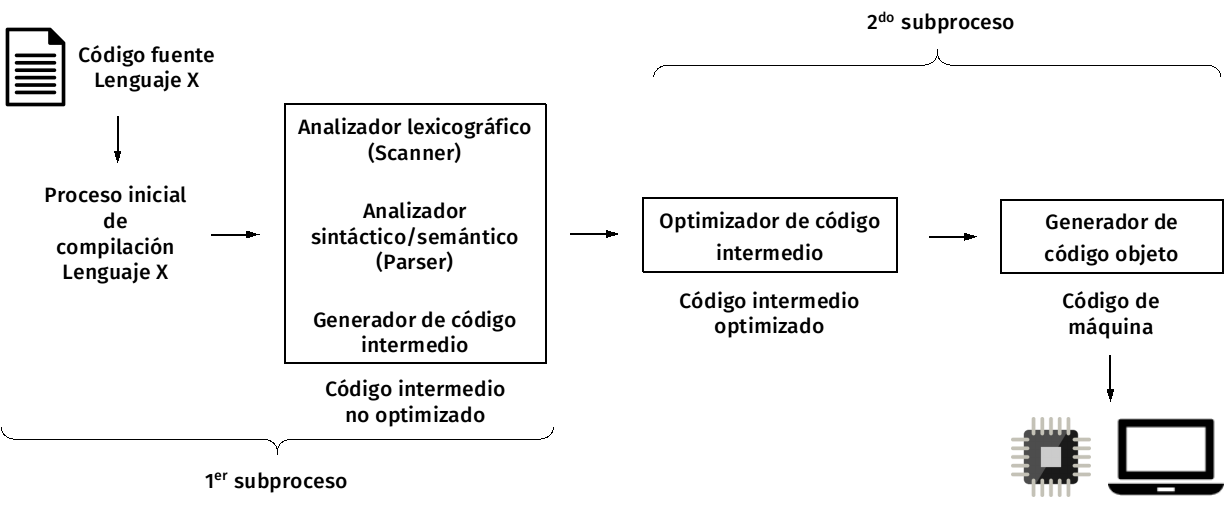
\includegraphics[width=1\textwidth]{./resources/compilation_op.png}
    \caption{Diagrama de bloques del proceso de compilación}
   \end{figure}
\end{frame}
